\section{Methodology and Implementation}
% What were the methods used?
% How was the problem designed?
% Driving concepts
% Equations
% Figures

A modular, \acrfull{ABM} approach is ideal for solving the coupled,
physics-dependent supply chain problems involving material routing, facility
deployment, and regional and institutional hierarchies which arise in \Cyclus. Additionally, the choice
to build \Cyclus on open source libraries in modern programming languages
enables both remote and multiprocess execution on a number of platforms. This
section begins by describing the general design features that make \Cyclus both
flexible and powerful: cluster-ready software and dynamic libraries.  The
\gls{ABM} framework is then described, focusing on its implementation and benefits
in a fuel cycle context. A discussion of the
time-dependent treatment of discrete resources follows, focusing on the
\gls{DRE}. Support for users and developers via the \Cycamore library of
archetypes and the experimental toolkit are also presented.  Lastly, the methods
for quality assurance are outlined.

\subsection{Modular Software Architecture}
% Motivation for encapsulated plug-in architecture
% enables ecosystem, ease of contribution across institutions
% enables myriad levels of simulation fidelity
% enables FC analyses that can compare ‘apples to apples'

The architecture of \Cyclus allows developers to define nuclear fuel cycle
processes independent of the simulation logic. To achieve this, \emph{agents} are
developed which represent facilities, institutions, and regions comprising the
nuclear fuel cycle. These agents are created using the \Cyclus framework
\gls{API}, a set of functions and protocols which assist in agent development
and specify how agents should be defined.  This encapsulated `plug-in' design
choice provides two major benefits. First, analysts can take advantage of the
simulation logic \gls{API} and archetype ecosystem when they apply \Cyclus to
their specific problem.  A modeler can focus on creating or customizing
nuclear facility, institution, resource, and toolkit models within their
specific area of technical expertise. Second, because \Cyclus uses a modular
archetype approach, comparing two archetypes is straightforward. For example, if
an analyst would like to compare the effect of using different models to
determine the input fuel composition for fast reactors, fuel
fabrication archetypes can be developed and interchanged while keeping the rest
of the models used in the simulation fixed.

\subsubsection{Cluster-Ready Software}

Innovative approaches to designing and optimizing robust fuel cycle strategies can become available by leveraging modern parallel computing resources.  For example, large scale sensitivity analyses to quantify the dependence of fuel cycle outcomes on potentially hundreds of uncertain parameters would only be feasible in a massively parallelized environment.
However, many fuel cycle simulators rely on \gls{COTS} and Windows-only software that limits
performance on and compatibility with resource computing infrastructures. This
constrains the possible scope of simulations and increases the wall-clock time necessary to conduct parameterized sensitivity
analyses and other multi-simulation studies. \Cyclus, on the other hand, is
primarily written in \texttt{C++} and relies on
libraries supported by Linux and UNIX (including Ubuntu and OSX) platforms,
which are flexible and support parallelization.
Furthermore, the core infrastructure and related archetypes are free and
open source, BSD-3-clause licensed.  \Cyclus can therefore be easily deployed
on large computer systems, such as \gls{HTC} systems.

Cyclopts \cite{gidden_cyclopts_2015}, a proof of principle design and
implementation of a \Cyclus-enabled application on such a large computer system,
uses UW-Madison's HTCondor \gls{HTC} infrastructure to perform sensitivity
studies. Cyclopts has run over $10^5$ jobs, comprising more than 60,000 total
compute hours. The \gls{HTC} infrastructure has separately been utilized to
run and collect information from full \Cyclus simulations running in parallel
on $10^3$ machines reliably for order $10^5$ simulations.

\subsubsection{Dynamically Loadable Libraries}

The \Cyclus architecture encourages efficient, targeted contribution to the ecosystem of
archetype libraries.
With \Cyclus, a researcher can focus on generating an archetype model within their
sphere of expertise while relying on the contributions of others to fill
in the other technologies in the simulation.
Similarly, individual developers may explore different levels of complexity within their archetypes, including
wrapping other simulation tools as loadable libraries within \Cyclus.

\Cyclus achieves this behavior by implementing generic \glspl{API} and a
modular architecture via a suite of dynamically loadable plug-in libraries
(pictured in Figure \ref{fig:framework}). By anticipating the possible classes of
information required by the simulation kernel, the \Cyclus \glspl{API}
facilitate information passing between the plug-in agents and the core
framework.
Though common in modern software architecture, such a plug-in paradigm has not
previously been implemented in a nuclear fuel cycle simulator.
It allows the core \Cyclus framework to operate independently from the plug-in libraries, and the
dynamically loadable plug-ins to be the primary mechanism for extending \Cyclus'
capabilities independent of the core.

\begin{figure}[htbp!]
\begin{center}
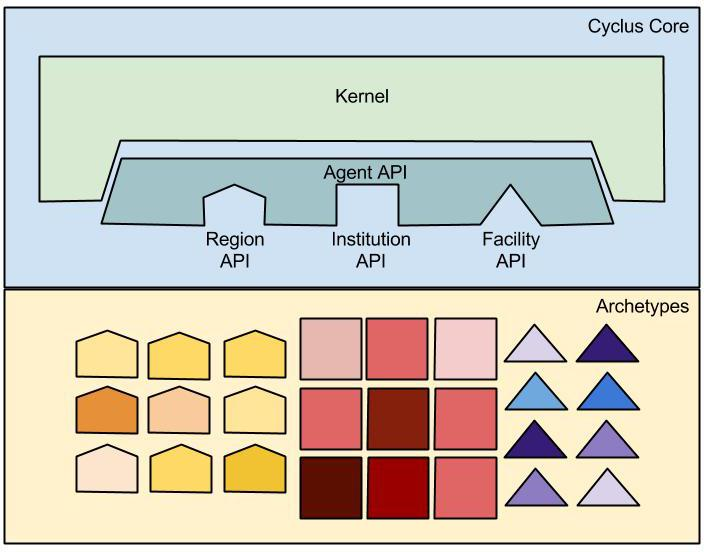
\includegraphics[width=\textwidth]{./images/framework}
\end{center}
\caption{The \Cyclus core provides \gls{API}s that abstract away the details in
the kernel and allow the archetypes to be loaded into the simulation in a modular
fashion.}
\label{fig:framework}
\end{figure}


An additional benefit is the ability for
contributors to choose different distribution and licensing strategies
for their contributions. Users and modelers control the accessibility of their archetypes and data sets (See Figure \ref{fig:modifiedopen}).
In particular, since the clean plug-in architecture loads libraries without any
modifications to the \Cyclus kernel, closed-source archetypes can be used with
the simulator alongside open source archetypes without transfer of sensitive information. This architecture
allows closed-source libraries (e.g., those representing sensitive nuclear
processes and subject to export control) to be developed and licensed privately.

\begin{figure}[htbp!]
\begin{center}
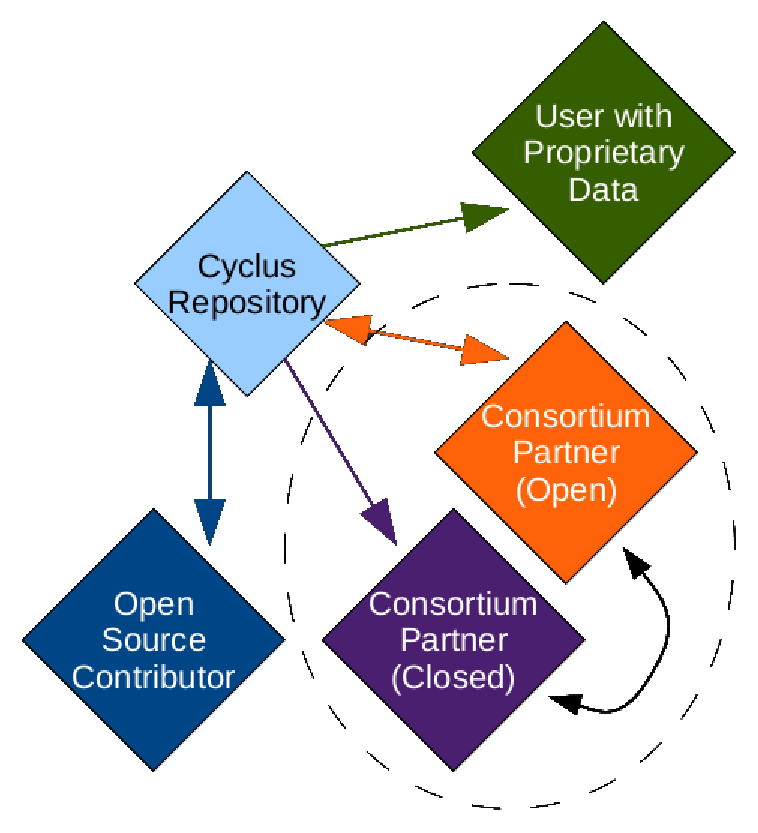
\includegraphics{./images/modifiedopen.eps}
\end{center}
\caption{The \Cyclus framework enables fully open, partially open, and fully
closed collaborations\cite{carlsen_cyclus_2014}.}
\label{fig:modifiedopen}
\end{figure}

Finally, dynamically loadable libraries enable \Cyclus to easily handle varying levels of simulation complexity. Hence a single
simulation engine can be used by both users interested in big-picture policy
questions as well as users focused on detailed technical
analyses. They merely choose their preferred level of modeling depth from among the
available libraries in the ecosystem.

\subsection{Agent-based Paradigm}
\label{sec:abm}
% superior detail in capturing simulation dynamics
% more flexible control over behavior
% describe Region/Institution/Facility hierarchy
% note importance of generic resource exchange paradigm

\Cyclus implements an \acrlong{ABM} paradigm. \gls{ABM} enables model
development to take place at an agent level rather than a system level. In the
nuclear fuel cycle context, for example, an analyst can design a reactor agent
that is entirely independent from a fuel fabrication agent. Defining the
behavior of both agents according to the
\gls{API} contract is sufficient for them to interact with one another as
bona fide agents in the simulation.  The two archetype libraries can be used in
the same simulation without any shared knowledge, allowing modelers to
construct a simulation from building blocks of many types and origins.

Furthermore, the \gls{ABM} paradigm is superior to the system dynamic approach used in
current simulators.
System dynamics is a popular approach for modeling nuclear fuel cycles
\cite{jacobson_vision_2009,van_den_durpel_daness_2009,guerin_impact_2009,guerin_benchmark_2009}.
Formally however, system dynamics models are simply a strict subset of agent-based models
\cite{macal_agent-based_2010}.
That is, any system dynamics model can be translated
into an agent-based model.
\gls{ABM} techniques therefore enable a broader range of simulations in a more
generic fashion.

\subsubsection{Agent Interchangeability}\label{sec:interchangeability}

% (OO, cpp, xml, backends, inheritances, mixins, generic apis, etc.)

\gls{ABM} is inherently object-oriented because agents represent discrete,
independently acting objects.  Figure \ref{fig:framework} illustrates the
modular nature of \Cyclus archetypes.  The core of the \Cyclus simulator creates
a set of classes on which agent plug-ins are based.  Agent plug-ins utilize the
generic core \gls{API} to interact with one another.  For example, they use the
resource exchange paradigm \gls{API} for trading resources with one another.

Due to this plug-in architecture,
implementations of agents in a given scenario can be easily
interchanged. Critically, this novel functionality enables the comparison
between agent implementations. For example, a low-physics-fidelity
implementation of a reactor can be compared to an implementation with higher
physics fidelity, allowing an analyst to discern the effect of reactor physical
fidelity on a given fuel cycle.

Interchangeability is accomplished by providing \glspl{API} that define agent-to-agent
interaction and agent-to-environment interaction, primarily through the
\Class{Agent} and \Class{Trader} interfaces. Figure \ref{fig:agent_uml} shows
the ``inheritance'' structure of the \Class{Agent} class in a \gls{UML} diagram
format. It shows how the \Class{Agent} interface
provides a notion of parent-child hierarchical relationship, where parents can
choose to \textit{deploy} child agents and \textit{decommission} child
agents. For the archetype developer, this interface provides enormous power
very simply. The \gls{API} provides the \Class{Agent} with helpful functionality for
interacting with the \Cyclus simulation kernel while abstracting away unnecessary
detail.

\begin{figure}[htbp!]
\begin{center}
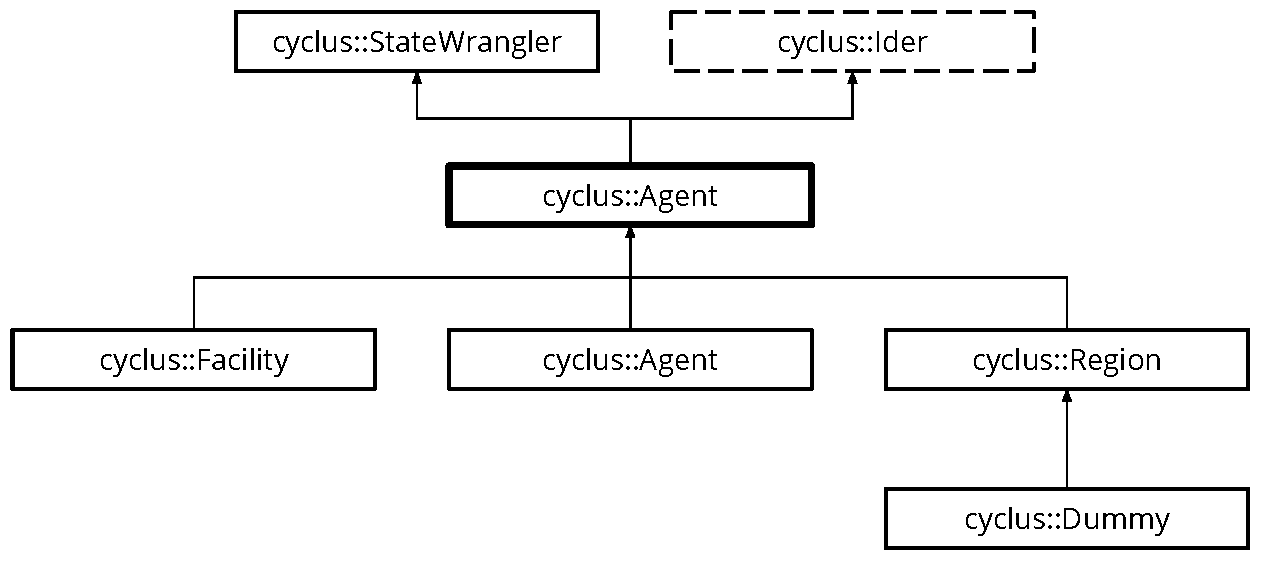
\includegraphics[width=0.5\textwidth]{./images/agent_uml}
\end{center}
\caption{The inheritance in \Cyclus classes, such as the \Class{Agent},
\Class{Facility}, \Class{Institution}, and \Class{Region} classes, abstract away
unnecessary details while exposing powerful functionality. In the above
example, the \Class{Dummy} archetype simply inherits from \Class{Region} in
order to become a bona fide Region-type \Class{Agent}.}
\label{fig:agent_uml}
\end{figure}

In this way, a researcher can directly compare two different reactor modeling
implementations (perhaps the imaginary classes \Class{DetailedReactor} and \Class{SimpleReactor})
simply by exchanging the two corresponding archetypes. That is, two reactor
archetypes both inheriting from the \Class{Facility} class are indistinguishable
from a simulation perspective.  This can be done with any agent type, where agents can be ``Regions,'' ``Institutions,'' or ``Facilities.''

\subsubsection{Regions, Institutions, and Facilities}

\Cyclus provides a novel representation of entities in the nuclear fuel cycle
that reflects the reality in international nuclear power: facilities implementing individual fuel cycle technologies, institutions managing those facilities, and regions providing geographical and political context for institutions and facilities. While
few simulators have provided any notion of static regional
effects \cite{huff_next_2010,juchau_modeling_2010}, \Cyclus allows for both regions and institutions to be first-class
agents in simulated fuel cycles. The fundamental interactions for each entity are implemented in a corresponding
archetype class in \Cyclus, i.e., the \Class{Region} class, \Class{Institution}
class, and \Class{Facility} class. Archetype developers can then build on the
provided functionality by inheriting from the appropriate class.
\Cyclus implements a \gls{RIF} relationship through the
parent-child hierarchy described in \S \ref{sec:interchangeability}, where
regions are the parents of institutions which are, in turn, the parents of
facilities. In other words, \gls{RIF} hierarchies form a directed acyclic graph (DAG),
with regions as root nodes and facilities as leaf nodes.

Two primary consequences arise from this structure. First, institutions are
nominally responsible for deploying and decommissioning facilities. Accordingly, advanced
logic regarding building and decommissioning can be implemented on top of
those behaviors inherited from the
\Class{Institution} interface. Second, the \Class{Facility} class implements the
\Class{Trader} interface, and thus institutions and regions, respectively, can
adjust the resource flow preferences of their managed facilities. Importantly,
this capability allows for the modeling of preferential regional trading
of resources (e.g., tariffs) as well as preferential institutional trading
(e.g., long-term contracts).

\subsection{Discrete Objects}
% enables more realistic models and metrics
% material routing metrics
% shadow fuel cycles
% etc.

\Cyclus models facilities, institutions, regions, and resources as discrete
objects. A discrete resource model allows for a range of modeling granularity. In the
macroscopic extreme, it is equivalent to time-stepped continuous flow. In the
microscopic extreme, the model is capable of representing arbitrarily small
material objects at isotopic resolution. In this way, \Cyclus is
applicable across the full range of modeling fidelity.

Fleet-based, lumped-material models do not distinguish between discrete facility
entities or materials. However, some questions require resolution at the level
of individual facilities and materials.  As a result, many detailed performance
metrics cannot be captured with previously existing fleet-based models. For all
of the reasons that the \gls{ABM} paradigm in \ref{sec:abm} enables novel
simulations, multiple use cases require that these agents, such as the regions,
institutions, and facilities in \Cyclus, must be represented as discrete
objects. For instance, tracking of individual shipments is only viable if materials and
resources are tracked as discrete objects.

\subsubsection{Resources and Materials}
% Resources, Materials (note isotope tracking, decay behavior)

Another such use case seeks to capture system vulnerability to
material diversion. Provenance and trade-history of distinct materials is the fundamental
information unit in such studies, and so this type of analysis requires
 discrete simulation of a
target facility and the individual materials modified within it.
Material risk analysis, therefore, demands that both facilities and materials
should be discretely modeled objects like those in \Cyclus.

In \Cyclus, agents can transfer discrete resource objects among one another.
Cyclus supports two types of resources:

\begin{itemize}

  \item materials: these represent typical nuclear materials with
      nuclide compositions;

  \item products: these can represent any user-defined measure: carbon
      credits, build permits, employees, etc..

\end{itemize}

All operations performed on every resource object (splitting, combining,
decay, etc.) are tracked in detail as they are performed.  This information
includes the agent that created each resource when it was introduced into the
simulation.  The parentage of each resource is also tracked. This makes it
possible to follow the history of resources as they are transferred between
agents.

The \Cyclus kernel has built-in experimental support for decay calculations.
Materials store the time since their last decay and agents are free to
invoke the decay function on them as desired to decay them to the current
simulation time. \Cyclus can currently operate in 3 decay modes, with 1 additional
mode likely to be added in a future release:

\begin{itemize}
    \item "manual" (currently implemented) is the default mode
        where agents decay materials when requested by an archetype,
    \item "never" (currently implemented) globally turns off all decay.
        The Material decay function does nothing,
    \item "lazy" (currently implemented) decays material automatically whenever
         its composition is observed (e.g. when an agent queries information
         about a material's $^{239}$Pu content),
    \item "periodic" (future) automatically decays all materials in a
        simulation with some fixed frequency.
\end{itemize}


When decay is invoked, a material checks to see if it contains any nuclides with
decay constants that are significant with respect to the time change since the
last decay operation.  If none of the decay constants are significant, no decay
calculation is performed and the material remains unchanged.  This error does
not accumulate because the next time the material's decay function is invoked,
the time change will be larger.

\Cyclus has no notion of ``tracked'' versus ``untracked'' nuclides.  In
\Cyclus, the composition of a material is represented by an arbitrarily large
list (potentially thousands) of nuclides.  Agents are free to treat nuclides
present in materials any way they please - including ignoring them.  It is the
responsibility of archetype developers to choose how to handle potentially
full-fidelity compositions.

In large simulations, many material objects may change frequently.  Material
decay can also contribute significantly to such changes.  In order to help
avoid unnecessary runtime performance and database size impacts, compositions
in \Cyclus have some special features.  In particular, compositions are
immutable once created. This allows multiple material objects to hold
references to the same composition safely.  Additionally, new compositions
resulting from decay are cached and used to avoid redundant decay
calculations.  Figure \ref{fig:compositions} illustrates how this decay
history cache works. Composition immutability in concert with decay history
caching help eliminate many redundant calculations in addition to reducing the
total number of composition entries recorded in the database.


\begin{figure}[htbp!]
\begin{center}
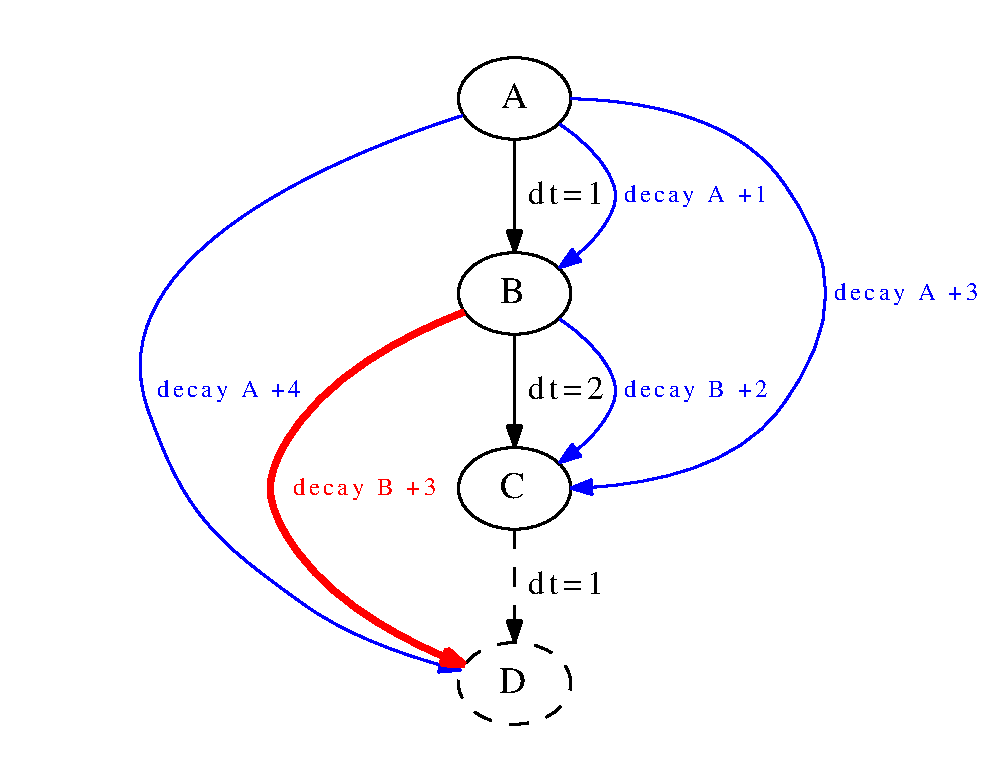
\includegraphics{./images/compositions}
\end{center}
\caption{
A simple decay line cache holding compositions A, B, C, and a
yet-uncomputed composition D.  B comes from decaying A 1 time step.  C comes
from decaying B 2 time steps, etc.  Black represents the cache for this
particular composition chain. Blue indicates decay operations that can be
satisfied by cache lookups.   If A needs to be decayed 1 time step (A +1), a
quick lookup returns the previously computed B.  Decaying B 3 time steps
requires a decay calculation to compute a new composition D, but subsequent
requests such as decaying A 4 time steps will not require any recalculation.
}
\label{fig:compositions}
\end{figure}

% although this abbreviation is provided by the glossary capability, I think
% the DRE is so important that it should be redefined here.

\subsubsection{Dynamic Resource Exchange (DRE)}

The \Cyclus simulation paradigm allows discrete agents, based on archetypes
about which the kernel has no knowledge, to enter the simulation at arbitrary
times and trade in discrete resources. These resources are not defined \textit{a
  priori}. Therefore, the logic engine defining resource interaction mechanisms
among agents is crucial. The \gls{DRE} is that critical logic engine on which
\Cyclus simulations are built.  Supporting the general \Cyclus philosophy,
facilities are treated as black boxes and a supply-demand communication
framework is defined.

The \gls{DRE} consists of three steps: supply-demand information
gathering, resource exchange solution, and trade execution. Importantly, each
step is agnostic with respect to the exchange of resources in question, i.e.,
the same procedure is used for both Materials and Products.

The information-gathering step begins by polling potential consumers. Agents
define both the quantity of a commodity they need to consume as well as the
target isotopics, or quality, by posting their demand to the market exchange as
a series of \textit{requests}. Users may optionally parameterize the agent to
associate a collection of demand constraints with each collection of requests.
Collections of requests may be grouped together, denoting \textit{mutual}
requests that represent demand for
some common purpose. For example, a reactor may request \gls{UOX} and \gls{MOX} fuel
mutually, indicating that either will satisfy its demand for fuel.

Suppliers then respond to the series of requests with a \textit{bid}. A bid
supplies a notion of the quantity and quality of a resource to match a
request. Suppliers may add an arbitrary number of constraints to accompany
bids. For example, an enriched \gls{UOX} supplier may be constrained by its current
inventory of natural uranium or its total capacity to provide enrichment (SWUs), and
attach such constraints to its bids.

Any potential resource transfer, i.e., a bid or a request, may be denoted as
\textit{exclusive}. An exclusive transfer excludes partial fulfilment; it must
either be met fully or not at all. This mode supports concepts such as the
trading of individual reactor assemblies.  In combination with the notion of
mutual requests, complex instances
of supply and demand are enabled.

Finally, requesting facilities, institutions and regions may apply
\textit{preferences} to each potential request-bid pairing based on the proposed
resource transfer. Facilities can apply arbitrary complex logic to rank the bids
that they have received, whether based on the quantity available in each bid or
on the quality of each bid, and the consequent implications of the physics behavior
of that facility. In addition, an institution can apply a higher preference to a
partner to which it is congenial; similarly, a region may negate any transfers
of material which have a higher uranium enrichment than is allowable.

Given a full definition of supply and demand, the \gls{DRE} may be solved either
optimally using a mathematical program or approximately by a simulation-based
heuristic \cite{gidden_agent-based_2014}. If any trade is denoted as exclusive, e.g., if an
analyst desires an assembly-fidelity model, then either a heuristic must be used
or exchanges must be represented as a \gls{MILP}. If no exclusive trades exist,
a \gls{LP} model may be used. In practice, \glspl{LP} solve much faster than
\glspl{MILP}. However, both capabilities exist in \Cyclus in order to
provide users with the desired level of fidelity.

Trades between agents are initiated by the \Cyclus kernel after a solution to
the \gls{DRE} is found. For each trade, the supplying agent is notified of its
matched request and provides an associated resource to the exchange. All
supplied resources are then sent to the corresponding requesting agents.

In \Cyclus, the \gls{DRE} is executed at each time step. Therefore, if a
facility's request for a resource is not met at a given time step, it may offer
a request in the following time step. Because agent behavior may change
arbitrarily, the exchange executed at any given time step may be unique in a
simulation.

The \gls{DRE} is a novel simulation concept in the nuclear fuel cycle domain. It
provides a flexible supply-demand infrastructure, supporting dynamic flows of
resources between agents, even as those agents enter and leave the simulation, and
even when those agents are defined by archetypes of arbitrary complexity. Trading
between agents can be affected by both the
proposed quality of a resource and agent relationships through the use of
preferences. Accordingly, a wide range of possible effects can be
modeled, from capacity-limited fuel supply to international trade agreements.

\subsection{Simulation Support}
So that users and developers can build working simulations in the shortest time
possible, the \Cyclus ecosystem provides fundamental building blocks: basic
archetypes and a toolkit of commonly needed functions.  The \Cycamore library
provides a suite of fundamental Region, Institution, and Facility archetypes,
while the \Cyclus toolkit provides assistance to developers.

\subsubsection{Cycamore}
% base modules

\Cycamore \cite{carlsen_cycamore_2014}, the \Cyclus additional module
repository, provides a fundamental set of agent archetypes for basic simulation
functionality within \Cyclus.  Since \Cyclus relies on external
archetypes to represent the agents within a simulation, \Cycamore provides the
basic archetypes a new user needs to get started running simple simulations.
These archetypes support a minimal set of fuel cycle simulation goals and
provide, by example, a guide to new developers who would seek to contribute
their own archetypes outside of \Cycamore.

As of version 1.0, \Cycamore contains one region archetype, two institution
archetypes, and four facility archetypes. Short descriptions of these functions
can be found in Table \ref{tab:cycamore}.


\begin{table}[h]
\centering
\begin{tabularx}{\textwidth}{|r|l|X|}
\hline
\textbf{Entity} & \textbf{Archetype} & \textbf{Functionality} \\
\hline
Facility & BatchReactor & A reactor model that handles batch refueling, based on pre-determined recipes of compositions. \\
Facility & Source & This facility generates material of the composition and commodity type specified as input.  \\
Facility & Sink & This facility is capable of accepting a finite or infinite quantity of some commodity produced in the simulation. \\
Facility & EnrichmentFacility & This facility enriches uranium at a specified capacity. \\
Institution & ManagerInst & The manager institution manages production of commodities among its facilities by building new ones as needed. \\
Institution & DeployInst &  This institution deploys specific facilities as defined explicitly in the input file. \\
Region & GrowthRegion & This region determines whether there is a need to meet a certain capacity (as defined via input) at each time step. \\
\hline
\end{tabularx}
\caption{The Archetypes in \Cycamore seek to cover a large range of simple simulation use cases \cite{carlsen_cycamore_2014}.}
\label{tab:cycamore}
\end{table}

As illustrated in
Figure \ref{fig:simplesim}, the current \Cycamore release provides basic
functionality enabling simple fuel cycle analyses. As future contributions are
vetted, the capabilities in \Cycamore may grow.

\begin{figure}[htbp!]
\begin{center}
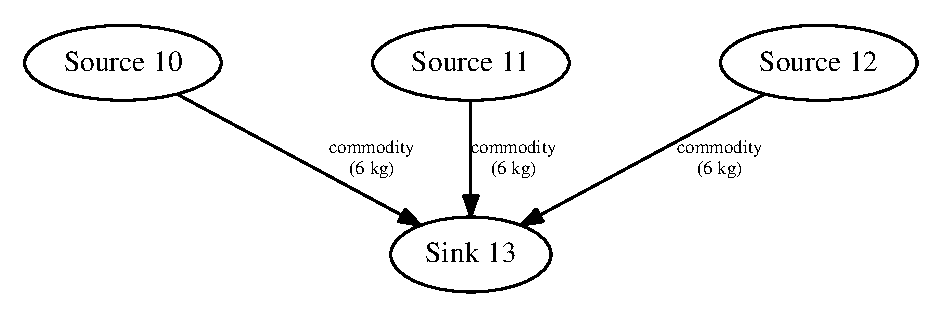
\includegraphics{./images/simplesim}
\end{center}
\caption{Material flows through a simple dynamic simulation created with only the simplest \Cycamore archetypes, \Class{Sink} and \Class{Source}.}
\label{fig:simplesim}
\end{figure}

\subsubsection{Toolkit}

In addition to the core functionality of the \Cyclus kernel, which is focused on
the set of capabilities needed to implement an agent-based simulation
with \gls{DRE}, a toolkit is provided to assist developers
and users with related simulation and nuclear engineering tasks. The toolkit is
an actively developed part of \Cyclus, with a primarily forward-looking
focus on supporting interesting \textit{in situ} metric analysis tools.

\paragraph{Simulation Tools}

A series of utility classes are provided to support demand-constrained agent
facility deployment. For example, symbolic function representations of linear,
exponential, and piecewise functions are supported via the
\Class{SymbFunctionFactory} class. Such functions are used with other toolkit
classes to determine commodity demand (e.g., power demand) from user input. Four
mix-in classes provide the basis for in-simulation deployment determination:
\Class{CommodityProducer}, \Class{CommodityProducerManager}, \Class{Builder},
\Class{BuildingManager}. The \Class{CommodityProducer} class provides an
interface for querying the \textit{prototypes} which have the
capacity to produce a given commodity. The \Class{CommodityProducerManager}
provides an interface for registering \Class{CommodityProducer}s and querying
the current capacity (supply) of a commodity. The \Class{Builder} class provides
an interface for querying which prototypes can be built and interacts with the
\Class{BuildingManager}, which orders prototypes to be built. The
\Class{BuildingManager} uses a simple minimum cost algorithm to determine how
many of each prototype, $y_i$, to build given a demand ($\Phi$), capacities
($\phi_i$), and costs ($c_i$). Here $i$ indexes $I$ available prototypes which perform a similar function, and the demand, capacity and cost carry prototype-specific units which are defined by the developer.

\begin{equation}
\begin{aligned}
 \min & \sum_{i=1}^{N}c_i y_i \\
 s.t. & \sum_{i=1}^{N}\phi_i y_i \ge \Phi \\
      & y_i \in [0,\infty) \:\: \forall i \in I, \:\: y_i \:\: \text{integer}
\end{aligned}
\end{equation}

\paragraph{Nuclear Engineering Tools}

The \Cyclus toolkit provides two useful interfaces for querying physical parameters of \Class{Material}
objects. First, the \Class{MatQuery} module
provides a basic querying \gls{API}, including the atom and mass fractions of
nuclides, the number of moles of a nuclide in a material, etc. (i.e., a
\Class{Composition}), in a material. The
\Class{Enrichment} module provides an \gls{API} for determining enrichment-related
parameters of a material, including the separative work units (SWU) and natural
uranium required to enrich a material provided knowledge of feed, product, and tails
assays.

\paragraph{Toolkit Extensions}

In addition to those that already exist, new tools will
emerge from the archetypes developed by the community. As these tools gain adoption between projects and demonstrate their
utility to the developer community, they will be considered for screening and
adoption into the kernel as toolkit extensions. Likely extensions include

\begin{itemize}
\item fuel cycle metrics calculators,
\item supportive data tables,
\item policy models,
\item and economic models.
\end{itemize}

\subsection{Quality Assurance}
% Organize this section according to major topics
% give each topic a section heading in boldface.
% try to cover the major common points :
%
% problem design
% methods of measurement
% supporting models
% supporting data
% simulations run
% results

% Just write the section headings for each part and indicate what goes in that
% section with words :
%
% heading
% figures (with captions)
% schematics (with captions and footnotes)
% equations
% tables

% What does it mean?
% What did I actually test?
% What were the results?
% Did the work yield a new method?
% Did the work yield new knowledge?
% What measurements did I make?
% How were these measurements characterized?
% What methods were used?
% What were the results?
% How were the measurements made and characterized?

Simulation science - like experimental science - must distinguish trustworthy
results from untrustworthy ones.
Charles Babbage famously articulated this, ``On two occasions I have been asked,
`Pray, Mr. Babbage, if you put into the machine wrong figures, will the right
answers come out?' ... I am not able rightly to apprehend the kind of confusion
of ideas that could provoke such a question.'' \cite{babbage_passages_2011}.
A simulator must assure correctness and guard against the \emph{garbage
in, garbage out} phenomenon.

Multiple strategies, collectively known as \emph{\gls{QA}}, have
been invented to mitigate structural and algorithmic errors
in software. These include \emph{\gls{VV}}
\cite{boehm_software_1989}, testing, and others.

Nuclear engineering software quality is often governed by \gls{NQA1}, an
\gls{ASME} specification
whose latest revision appeared in 2009 \cite{asme_nqa-1a-2009_2009}.
\Cyclus has adopted an \emph{agile} development process
\cite{larman_agile_2004},
interpreting \gls{NQA1} in a manner similar to the process adopted by the
\gls{DOE} within \gls{NEAMS} \cite{neams_nuclear_2013} or by the PyNE toolkit
\cite{biondo_quality_2014}.

Verification may be defined as the question, ``Is \Cyclus being built correctly?''
To answer this question, \Cyclus relies on software development best practices
such as testing,
documentation, version control, style guidelines, and continuous integration to
ensure reliability and reproducibility. These verification techniques are
discussed individually in the sections that follow.

Validation, in contrast,  may be defined as the question,
``Is \Cyclus the correct tool?''
Since \Cyclus is alone in its class as an agent-based fuel cycle simulator, longitudinal
validation is not possible. Nonetheless, code-to-code comparisons with fuel cycle
simulators that use other modeling paradigms are underway
\cite{huff_extensions_2014}. However, such
exercises are more likely to bring into relief the differences between the modeling
paradigms than supply substantial \gls{QA} and validation.

Sections \ref{sec:qa-testing}-\ref{sec:qa-ci} discuss in greater detail the software
development components that comprise the \Cyclus verification strategy.
Each of these on its own is a valuable addition to \gls{QA} but is cannot be the
entire answer to the requirements imposed by \gls{NQA1}. Taken together and strictly
adhered to, they present a fortress to protect against poorly designed or otherwise undesirable code.


\subsubsection{Testing}
\label{sec:qa-testing}

Automated software \emph{testing} is the first line of defense against
errors in implementation. It also acts as an early warning sign if the
simulator does not work as intended on a new system.
Testing serves a critical role in \gls{QA} because it directly compares the
results of running software versus the expected behavior of the software.
In \Cyclus, three categories of tests are defined: unit tests, integration
tests, and regression tests.  It is important to note that before a proposed
code change is allowed into \Cyclus,  the change must be covered by a test, either new or existing, and all tests must pass.

\paragraph{Unit Tests}

Unit tests compare the results of the smallest code \emph{unit}, typically a
single function or a class.  \Cyclus uses the Google Test framework
\cite{inc_googletest_2008} as a harness for running unit tests. Sufficient unit
tests are required for any proposed change to the \Cyclus code base. Currently,
\Cyclus implements over 450 unit tests and \Cycamore implements 85.  These
cover approximately 65\% of their respective code bases, and these numbers are
expected to grow over time.

\paragraph{Integration Tests}

Integration tests combine multiple elements of the
\Cyclus interface and test that they work correctly with each other.  By analogy,
simply because the gears (units) are made correctly does not imply that the
clock (integration) will run smoothly, run at all, or give the correct time.
In \Cyclus and \Cycamore, integration tests are performed by running sample
simulations for scenarios that are sufficiently simple to predict the results
and verifying that results match those predictions. A set of standard input
files are run, then the output is inspected and compared via Nose
\cite{pellerin_nose_2007}, a Python test framework.  In this way, \Cyclus code
units are tested in the full context that they will be
executed. This category of testing is especially useful for ensuring that
major \Cyclus components are functioning as expected.

\paragraph{Regression Tests}

Regression tests ensure significant unintended changes do not
occur over the course of \Cyclus development. Such a change is called a
\emph{regression} because the new version is almost always wrong.
Regression tests are implemented similarly to integration tests.
In this category, however, the comparison is done against
the output of the same input file when run with a previous version of \Cyclus,
typically the last released version.
In some sense, regression tests are `dumb' in that they do
not care about the contents of a simulation being correct, only whether or not
it changed.

\subsubsection{Documentation}

All of the public interface (the \gls{API}) must be documented as required by
the \Cyclus \gls{QA} policy. This certifies that the intended goals of an
\gls{API} are communicated explicitly by the author in prose form.  In \Cyclus,
this information is aggregated together into static websites with the Doxygen
\cite{van_heesch_doxygen:_2008} and Sphinx \cite{brandl_sphinx_2014} tools, and
can be accessed at \url{http://fuelcycle.org}.

\subsubsection{Version Control}

Version control preserves the development history, or \emph{provenance}, of
source code files. \Cyclus uses a well-established \emph{distributed version
control} tool called git \cite{software_freedom_conservancy_git_2014} for this
purpose.  Distributed version control allows every
user to have complete local copy of the \emph{repository} (the version control
term for the collection of all possible histories).
One feature that git performs exceptionally well is \emph{branching}.
Branches are distinct pathways in the history that diverge from a mainline source
tree and then may be \emph{merged} back in. Multiple simultaneous
branches may exist at all points in time. Every change to the code is recorded
in the history, along with metadata such as the author, a timestamp, and an
accompanying message. Thus,
it is possible for \Cyclus to accurately replay the entirety of who did what to the
code when.

\Cyclus uses a strategy known as \emph{git flow}
\cite{kalliamvakou_code-centric_2014} to manage topical branches where
individuals develop code in parallel. All proposed software changes from
topical branches must have sufficient successful tests and comprehensive
documentation to be allowed into \Cyclus.  As an example, a schematic of the
development stages between reporting a bug and merging the fix is shown in
Figure \ref{fig:gitprocess}.

\begin{figure}[htbp]
\begin{center}
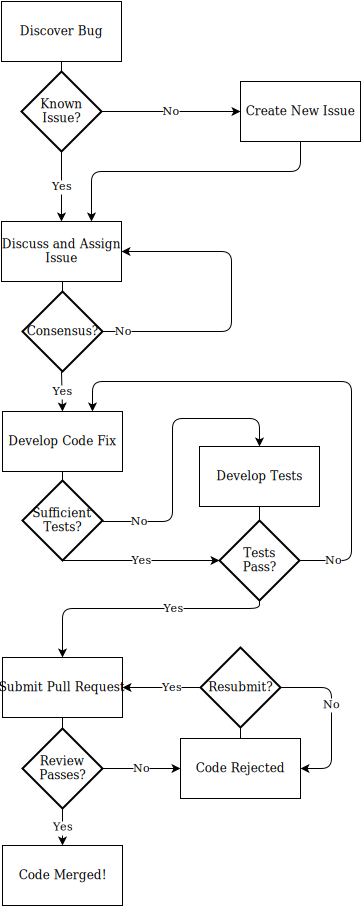
\includegraphics[height=0.6\textheight]{./images/gitprocess}
\end{center}
\caption{A version-control enabled process for finding, reporting, and fixing a bug
can take place within an issue tracker alongside multiple stages of software
testing and review. In the \Cyclus case, the final review stage includes unit,
regression, and integration testing as well as manual code inspection.}
\label{fig:gitprocess}
\end{figure}

The act of proposing a change is known as a \emph{pull request}. The main \Cyclus repository is
hosted remotely on the GitHub website \cite{dabbish_social_2012}. The online
mechanism for pull requests allows for code review by a member of the \Cyclus
core team, separate from the author, prior to any change being included. Non-members
of the \Cyclus development team are allowed and encouraged to submit and review
pull requests. However, only members of the \Cyclus core team are allowed to
merge in any changes and only after the \gls{QA} standards have been met. This
step has been repeatedly shown to improve code quality \cite{cohen_modern_2010}.

\subsubsection{Style Guide}

In any multi-person software project, there is a tension between how individuals
wish to write code. Every person tends to have their own custom style. To remedy this,
coding style guides are the software analogy to those for written language,
such as the Chicago Manual of Style. \Cyclus strictly enforces the use of the
Google C++ Style Guide \cite{weinberger_google_2008} for all software contributions.
This means that all developers of \Cyclus nominally write \Cyclus code in the same
way.  This homogenization may be a hurdle to new developers but ultimately
improves code legibility and, therefore, robustness \cite{cohen_modern_2010}.

\subsubsection{Continuous Integration}
\label{sec:qa-ci}

\emph{Continuous integration (CI)} is the idea that software should be tested and validated
as it is being developed, rather than as a final stage in a longer development
cycle.  Under \gls{CI}, every pull request (proposed code change) is tested independently immediately after
it is proposed. Such tests are run on all officially supported platforms.
\Cyclus uses a \gls{CI} platform called Polyphemus
\cite{scopatz_polyphemus_2014}. Polyphemus serves as an intermediary between GitHub pull requests on the front-end
and temporary \Cyclus servers on the back-end. These servers are hosted by
the Build \& Test Laboratory (BaTLab) \cite{uw_batlab_team_batlab_2014} at the University of
Wisconsin-Madison. Whenever a pull request is created, Polyphemus performs
the following actions:

\begin{enumerate}
    \item Copies \Cyclus with the proposed new code to BaTLab,
    \item Initializes Linux and Mac OSX servers,
    \item Builds \Cyclus on all platforms,
    \item Runs the complete \Cyclus test suite,
    \item Reports whether or not the above steps succeeded.
\end{enumerate}

Since these steps are performed for all incoming code, it is easy for the
\Cyclus core team to determine whether or not an individual pull request
actually works. This helps identify build and test problems prior to
broken code being allowed into the develop branch. \gls{CI} is a necessary
but not sufficient addition to the \Cyclus \gls{QA}
system: it keeps bad code out of \Cyclus. However, \Cyclus will always
require human eyes and hands to let good code in.
